\section{Results}
\label{sec:results}

\paragraph{Setup.}
For each application, we select 50 relevant Nemotron personas~\citep{nvidia2025nemotron} by embedding similarity between the application description and persona profiles to approximate the selection of real users whose backgrounds match the target application. Details persona selection are provided in \autoref{app:diversity}. We use \texttt{Claude Haiku 4.5}~\citep{anthropic2025haiku45} for persona-driven users, \texttt{GPT-4o mini}~\citep{openai2024gpt4omini} for chatbot applications, and cap chatbot conversations at eight turns.

% \begin{wrapfigure}[17]{r}{0.56\textwidth}
%     \centering
%     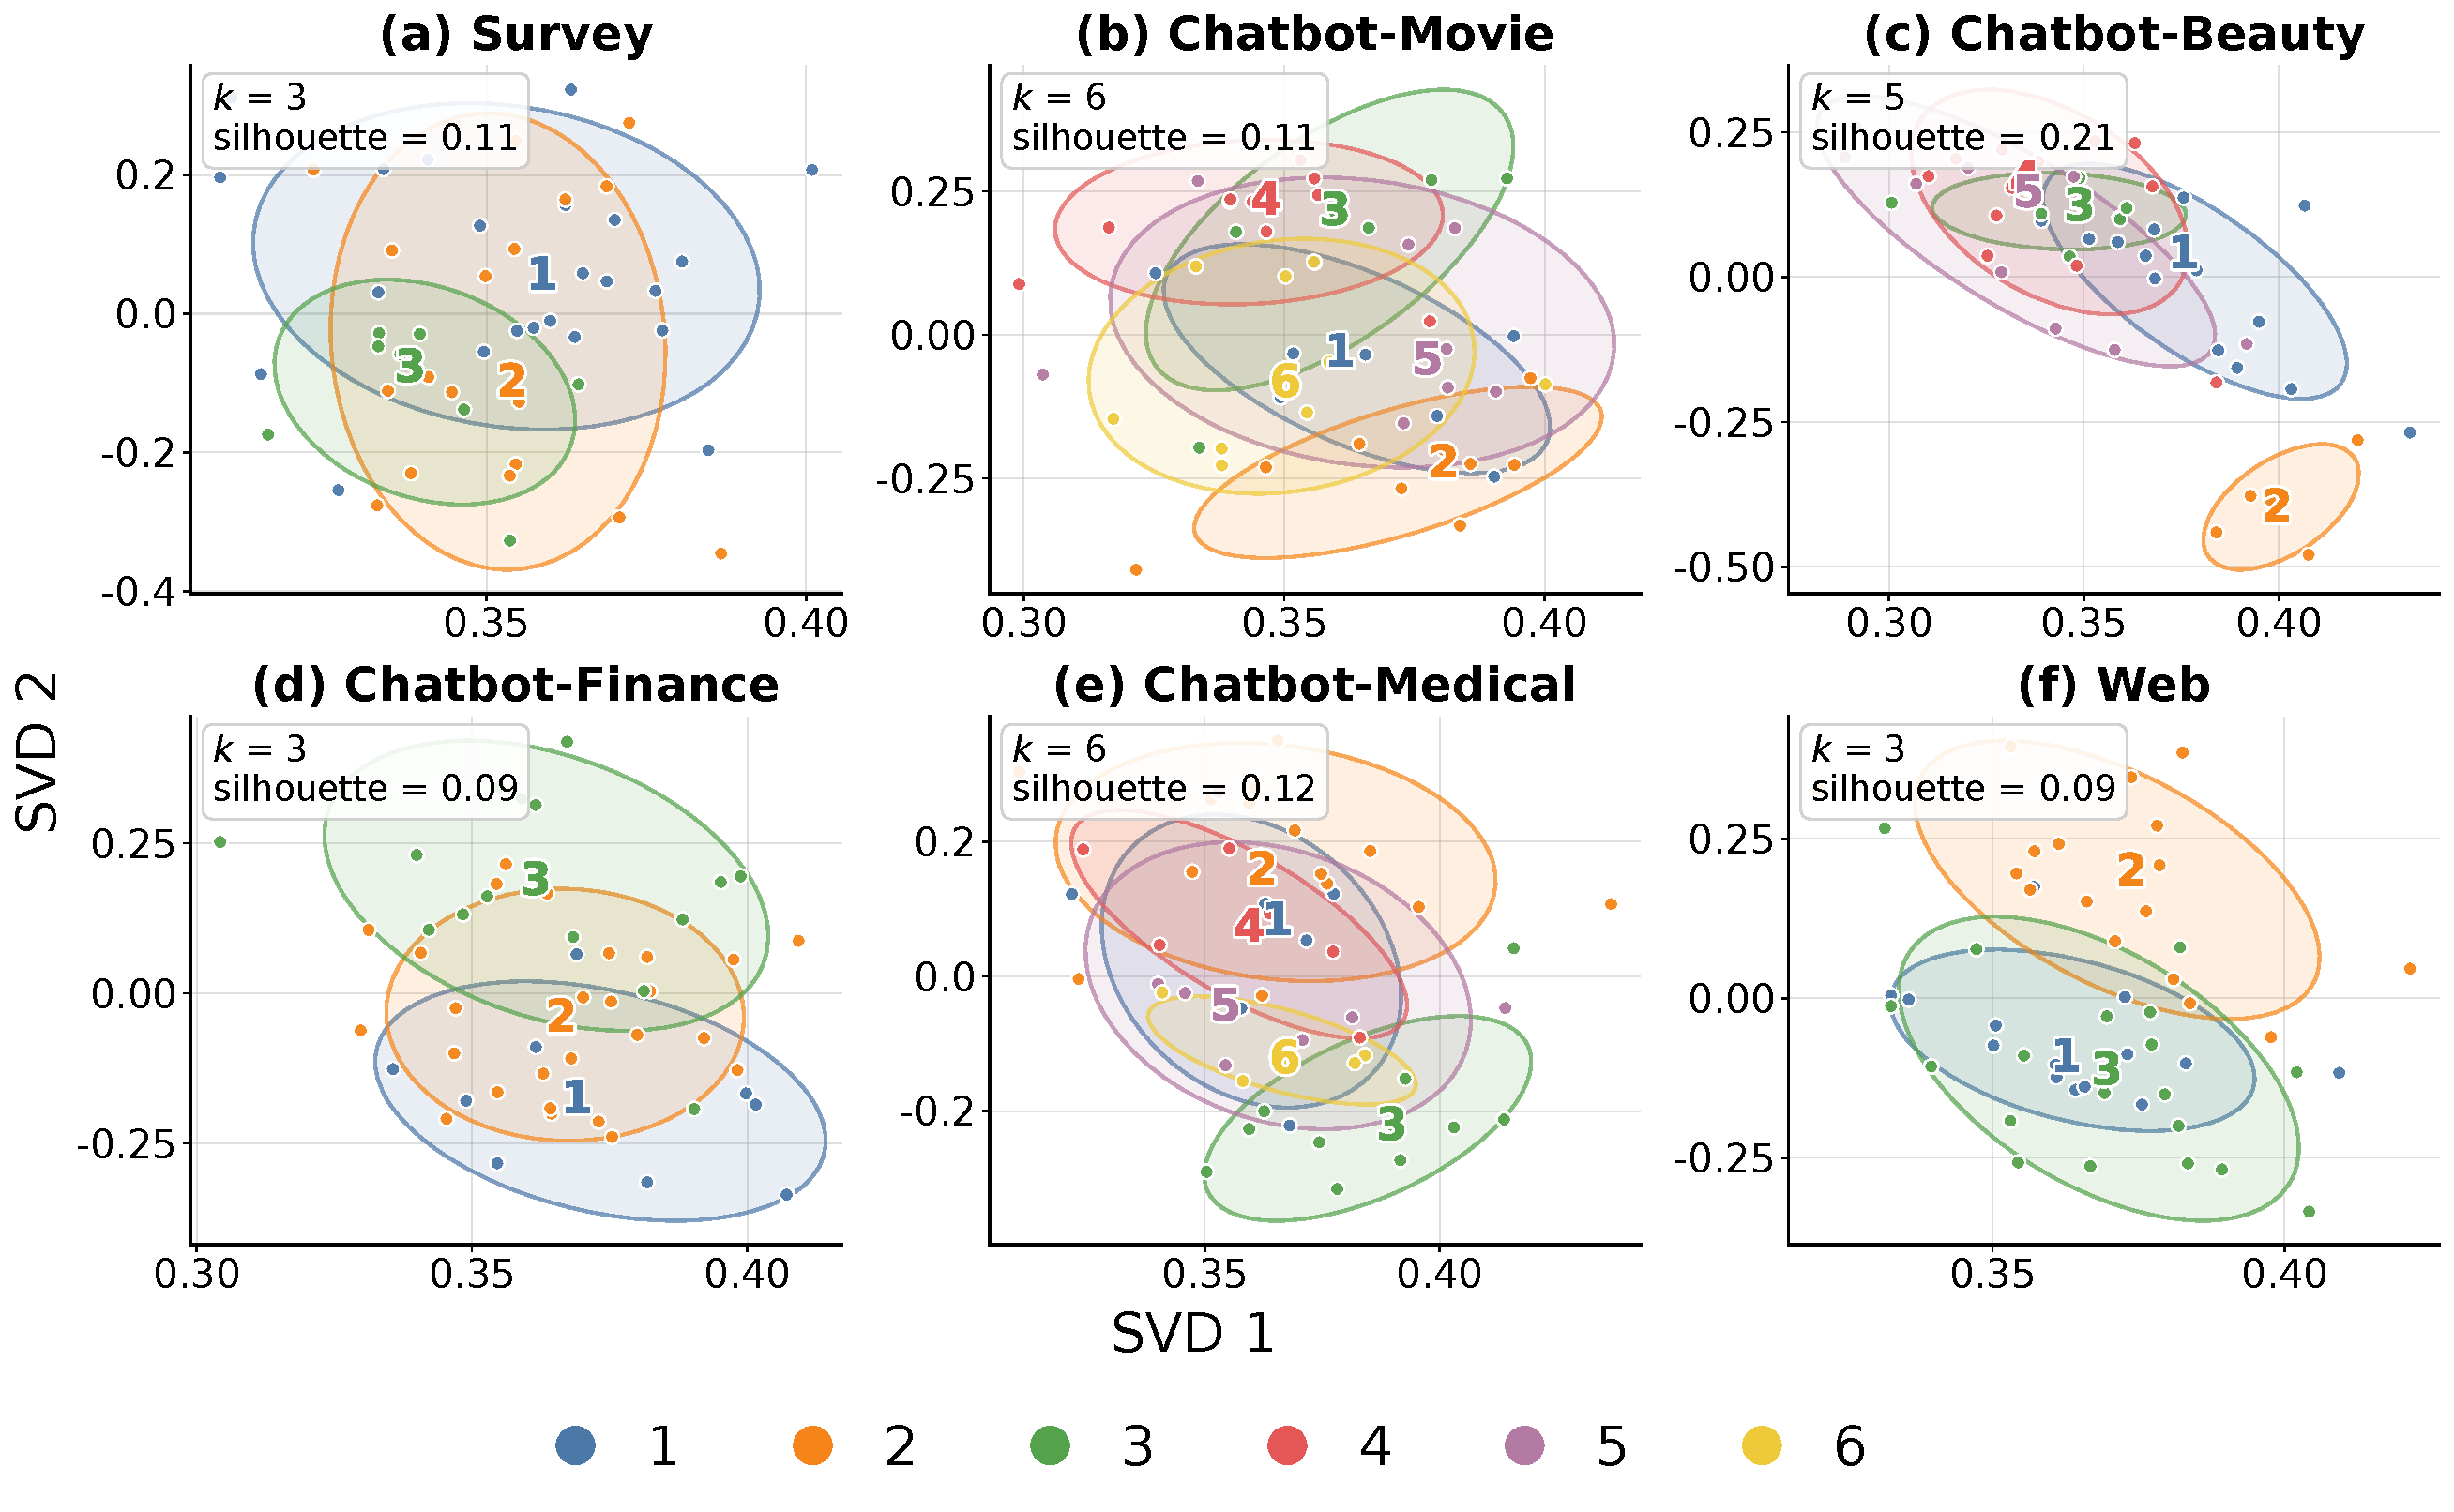
\includegraphics[width=0.56\textwidth]{figures/fig3_within_domain_clusters.pdf}
%     \caption{  \textbf{Diversity of selected personas.}
%   For each application instance, the 50 selected personas are clustered in a TF--IDF$\rightarrow$SVD space. The overlapping clusters show that application-relevant personas form soft thematic groups.}
%   \label{fig:within-clusters}
% \end{wrapfigure}

\begin{figure}[t]
    \centering
    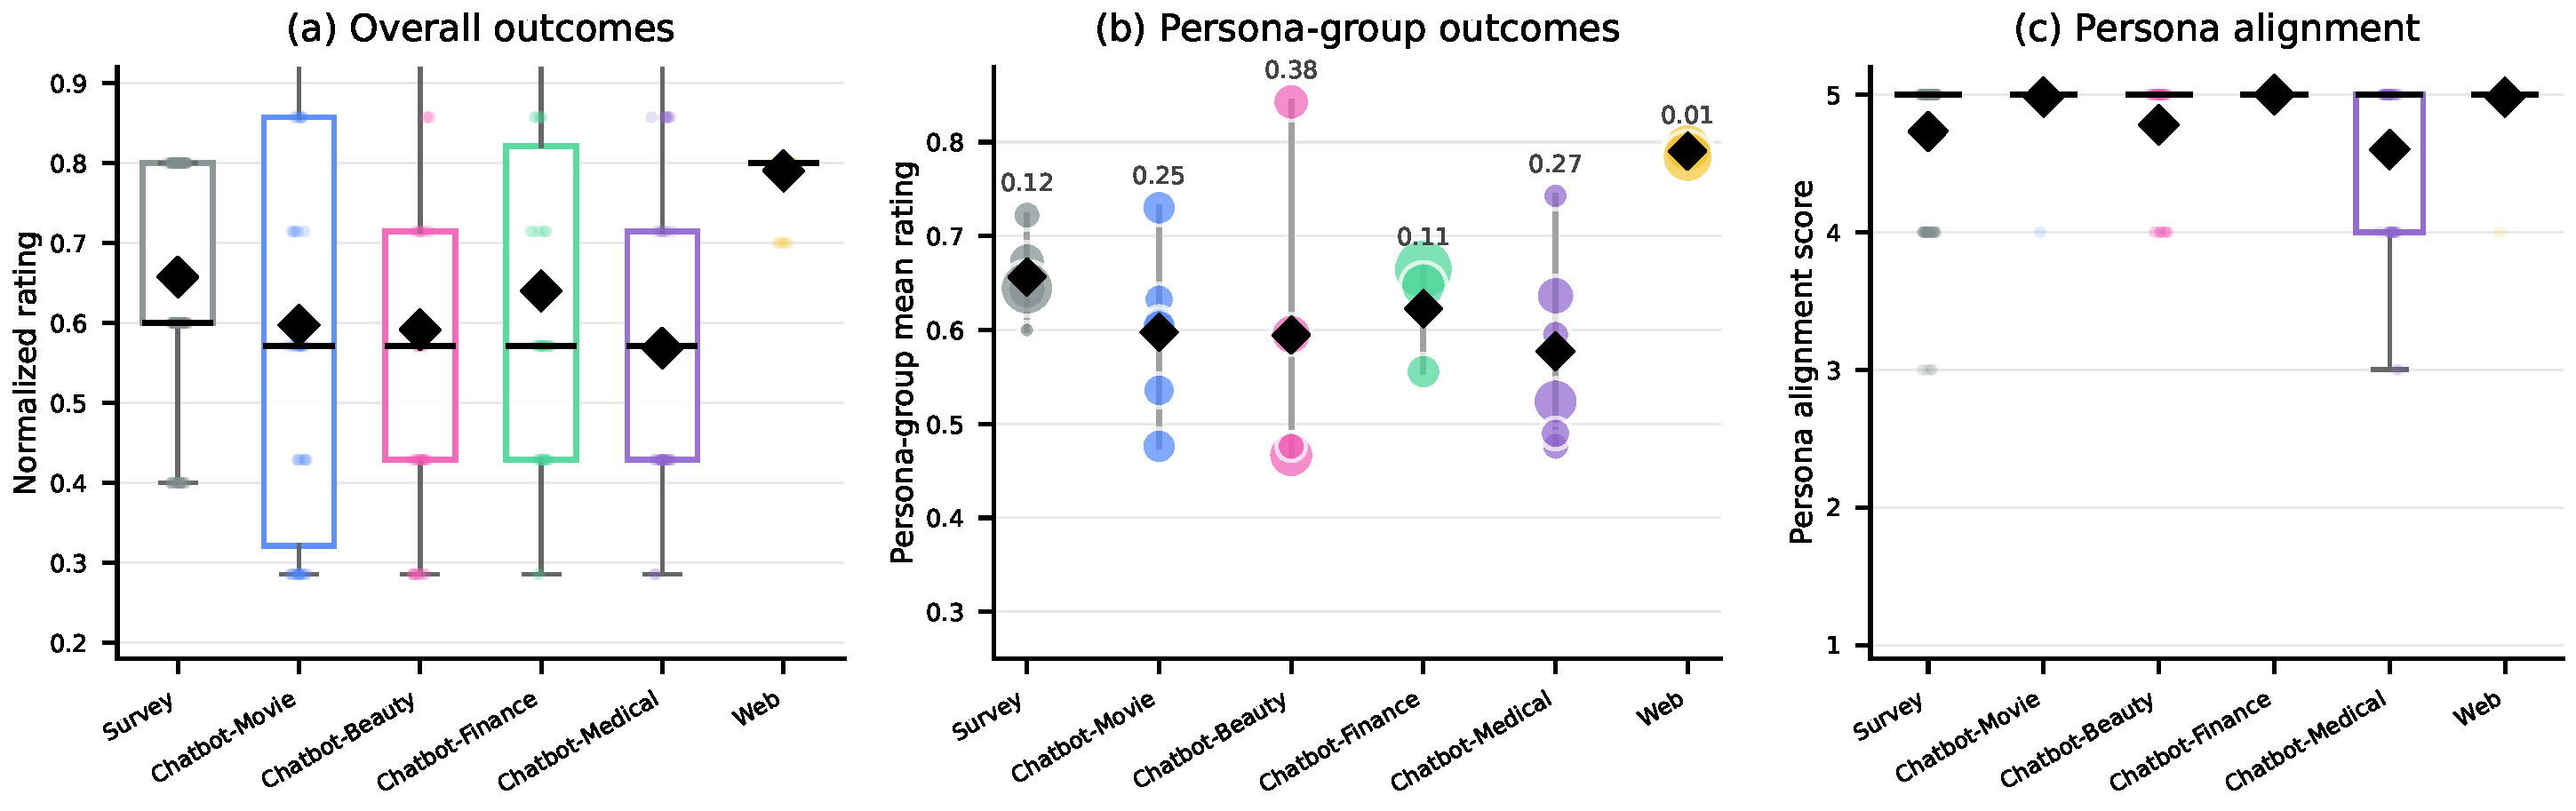
\includegraphics[width=0.80\linewidth]{figures/fig_results_components.pdf}
    \caption{
        \textbf{Results overview across survey, chatbot, and web settings.}
        Panel (a) shows normalized overall ratings, with diamonds marking application means. Panel (b) shows persona-group mean ratings; point size is proportional to group size, and numbers show the max--min group spread. Panel (c) shows persona alignment score distributions.
    }
    \label{fig:results-components}
\end{figure}

\begin{figure}[t]
    \centering
    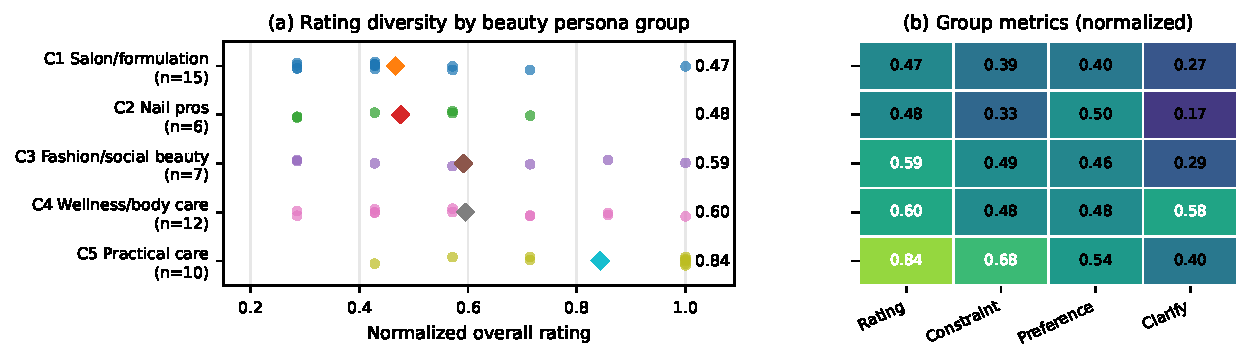
\includegraphics[width=0.98\linewidth]{figures/fig_beauty_persona_groups.pdf}
    \caption{
    \textbf{Beauty persona group results.}
    We group beauty users by shared persona traits: C1 salon and formulation users, C2 nail professionals, C3 fashion and social beauty users, C4 wellness and body care users, and C5 practical care users. Panel (a) shows normalized ratings for each persona, with diamonds marking group means. Panel (b) summarizes normalized group metrics. 
    %Professional groups rate lower when the system returns general consumer products, while practical care users rate higher when their needs fit the catalog.
    }
    \label{fig:beauty-groups}
\end{figure}

\paragraph{Overall result analysis.}
\autoref{fig:results-components}(a) analyzes simulated users' reported overall ratings. The chatbot tasks show moderate satisfaction with wider spread, because personas bring different goals, preferences, and domain knowledge into the interaction. Survey and web results are more concentrated, suggesting that structured survey responses and constrained web checkout produce more stable outcomes. Detailed results and representative interaction traces are provided in \autoref{app:results}.

\paragraph{Behavior differences across personas.}
\autoref{fig:results-components}(b) summarizes outcome variation across persona groups. Larger spreads in beauty, medical, and movie suggest that different user groups evaluate the same application differently, while survey, finance, and web show more similar group ratings. \autoref{fig:beauty-groups} shows the beauty case in more detail. We read the full persona profiles to name each group. Salon and formulation users (C1) and nail professionals (C2) give lower ratings because their goals often require professional sourcing, ingredient details, or salon inventory support. Practical care users (C5) give higher ratings because their needs better match the available product catalog.

\paragraph{Persona alignment analysis.}
We evaluate persona alignment with a human-judged 1--5 score that measures whether each simulated interaction is consistent with the assigned user persona. The judge considers the user's task goal, interaction trace, and final evaluation form. \autoref{fig:results-components}(c) shows that persona alignment remains high across survey, chatbot, and web applications. Lower scores appear more often in tasks where users need to express professional knowledge, personal constraints, or domain-specific concerns over multiple turns. Overall, these results suggest that \method produces persona-aligned simulations.

